\section{Preliminaries}\label{preliminaries}

Before stating Hilbert's 10th problem and proving its undecidability in
certain rings of algebraic integers, we remind the reader on some
notions of theoretical computer science and number theory, as well as
fix some notations.

\subsection{Preliminaries from theoretical computer
science}\label{preliminaries-from-theoretical-computer-science}

\subsubsection{Problems and Turing
machines}\label{problems-and-turing-machines}

In this section we closely follow the lecture notes on the subject by
@Mueller2016.

A \emph{(decision) problem} is a subset of the set of finite
\(\zer\)-\(\one\)-strings \(\lbrace \zer, \one \rbrace^*\) including the
empty string \(λ\). We call \(\lbrace \zer, \one \rbrace\)
\emph{alphabet} and its elements \emph{bits.}

One immediate objection against this definition is that not all problems
arise as subsets of these strings. However, such problems \(Q\) are
captured up to an encoding.

\[ \ulcorner . \urcorner : Q → \lbrace \zer, \one \rbrace^*\]

We usually do not concern ourselves with the details of this encoding.
However, the encoding should capture the structure of the problem.

Consider the problem of deciding wether a finite simple graph is
connected or not. If we fix each vertex set to be of the form
\(\lbrace 0, 1, …, n\rbrace\), then the set of all graphs can be encoded
as the set of the respective adjacency matrices written as a string

\[b_{00}b_{01} …b_{0n}b_{10}…b_{nn}\]

of length \((n + 1)^2\), where \(b_{ij} = \one\) if and only if the
vertices \(i\) and \(j\) are connected.

A \emph{Turing machine} \(\mathbb A\) on the \emph{alphabet}
\(A = \lbrace \sta, \emp, \zer, \one \rbrace\) is a tuple \((S, δ)\),
where \(\sstart, \shalt ∈ S\) is a finite non-empty set, called
\emph{set of states}, and

\[δ: S × A → S × A × \lbrace -1, 0, 1 \rbrace\]

is called \emph{transition function}. If \(δ(s, a) = (s', b, m)\), we
demand that the following axioms are satisfied.

\begin{enumerate}
\def\labelenumi{\arabic{enumi}.}
\tightlist
\item
  \(a = \sta\) if and only if \(b = \sta\).
\item
  If \(a = \sta\), then \(m ≠ -1\).
\item
  If \(s = \shalt\), then \(s' = \shalt\), \(a = b\) and \(m = 0\).
\end{enumerate}

Let \(\mathbb A = (S, δ)\) be a Turing machine. A \emph{configuration}
of \(\mathbb A\) is a triple \((s, j, c) ∈ S × ℕ × A^ℕ\). It reflects
the current state of \(\mathbb A\) the current position of its
\emph{head} and the content of its \emph{work-tape}.

A configuration of the form \((\shalt, 0, c)\) is called \emph{halting}.
A \emph{start configuration} is of the form \((\sstart, 0, c)\) such
that \(c(0) = \sta\) and there exists an \(n ∈ ℕ\) such that
\(c(i) = \square\) if and only if \(i > n\). This means that in a start
configuration the work-tape reads

\[\sta x_1 x_2 … x_n \square \square …\]

It will be very convenient to identify the finite string \(x_1…x_n\)
with this tape content.

We write \((s, j, c) \vdash_1 (s', j', c')\) and call \((s', j', c')\) a
\emph{successor configuration} of \((s, j, c)\) if there exists an
\(m ∈ \lbrace -1, 0, 1 \rbrace\) such that

\begin{enumerate}
\def\labelenumi{\arabic{enumi}.}
\tightlist
\item
  \(δ(s, c) = (s', c', m)\),
\item
  \(j' = j + m\), and
\item
  \(c'(ℓ) = c(ℓ)\) for all \(ℓ ≠ j\).
\end{enumerate}

This relation makes the set of all configurations of \(\mathbb A\) into
a directed graph. A \emph{run} of \(\mathbb A\) on \(x\) is a path in
this directed graph starting in the start configuration
\((\sstart, 0, x)\). A run of \(\mathbb A\) on \(x\) is \emph{halting}
or \emph{complete} if it reaches a halting configuration
\((\shalt, 0, y)\). In this case we write \(\mathbb A (x) = y\).

We will denote Turing machines using listings, where the fact that
\(δ_\text{a} (s_\text{state}, b) = (s_\text{state'}, c, m)\) is encoded
by

\begin{Shaded}
\begin{Highlighting}[]
\NormalTok{a }\StringTok{"state"}\NormalTok{ b }\FunctionTok{=}\NormalTok{ (}\StringTok{"state'"}\NormalTok{, c, m)}
\end{Highlighting}
\end{Shaded}

See the Appendix of this thesis on how to simulate these Turing machines
using the \emph{Haskell} programming language. We actually use valid
syntax of the \emph{glorious Glasgow Haskell compiler} in the listings.

Consider the Turing machine
\(\mathbb A_\text{add1} = (\lbrace \sstart, \shalt, s_\text{overflow}, s_\text{return} \rbrace, δ_\text{add1})\)
that adds \(1\) to a (possible zero-patched) binary representation of a
natural number \(n\).

\begin{Shaded}
\begin{Highlighting}[]
\CommentTok{-- start by entering the "overflow" state ...}
\NormalTok{add1 }\StringTok{"start"}    \CharTok{'§'} \FunctionTok{=}\NormalTok{ (}\StringTok{"overflow"}\NormalTok{, }\CharTok{'§'}\NormalTok{, }\DecValTok{1}\NormalTok{   )}
\CommentTok{-- ... and stay in this state, as long as you read only '1'-s}
\NormalTok{add1 }\StringTok{"overflow"} \CharTok{'1'} \FunctionTok{=}\NormalTok{ (}\StringTok{"overflow"}\NormalTok{, }\CharTok{'0'}\NormalTok{, }\DecValTok{1}\NormalTok{   )}
\CommentTok{-- if you read the first '0' or an empty cell replace it by '1'}
\CommentTok{-- and enter the "return" state to move the head to the first cell}
\NormalTok{add1 }\StringTok{"overflow"} \CharTok{'0'} \FunctionTok{=}\NormalTok{ (}\StringTok{"return"}\NormalTok{,   }\CharTok{'1'}\NormalTok{, (}\FunctionTok{-}\DecValTok{1}\NormalTok{))}
\NormalTok{add1 }\StringTok{"overflow"} \CharTok{'□'} \FunctionTok{=}\NormalTok{ (}\StringTok{"return"}\NormalTok{,   }\CharTok{'1'}\NormalTok{, (}\FunctionTok{-}\DecValTok{1}\NormalTok{))}
\CommentTok{-- we finish if we read '§' again or ...}
\NormalTok{add1 }\StringTok{"return"}   \CharTok{'§'} \FunctionTok{=}\NormalTok{ (}\StringTok{"halt"}\NormalTok{,     }\CharTok{'§'}\NormalTok{, }\DecValTok{0}\NormalTok{   )}
\CommentTok{-- ... continue to move to the right and don't change the cell}
\CommentTok{-- content. Here `b` matches '0' or '1'}
\NormalTok{add1 }\StringTok{"return"}\NormalTok{   b   }\FunctionTok{=}\NormalTok{ (}\StringTok{"return"}\NormalTok{,   b  , (}\FunctionTok{-}\DecValTok{1}\NormalTok{))}
\end{Highlighting}
\end{Shaded}

The complete run of \(\mathbb A_\text{add1}\) on \(\one\one\zer\one\)
cas be seen in {[}@fig:add1{]}.

\hypertarget{fig:add1}{}
\begin{figure}
\centering
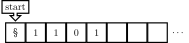
\includegraphics{res/turing_add1_1.svg}
\caption{\(δ(\sstart, \sta) = (s_\text{overflow}, \sta, 1)\)}
\end{figure}

\begin{figure}
\centering
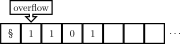
\includegraphics{res/turing_add1_2.svg}
\caption{\(δ(s_\text{overflow}, \one) = (s_\text{overflow}, \one, 1)\)}
\end{figure}

\begin{figure}
\centering
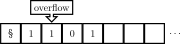
\includegraphics{res/turing_add1_3.svg}
\caption{\(δ(s_\text{overflow}, \one) = (s_\text{overflow}, \one, 1)\)}
\end{figure}

\begin{figure}
\centering
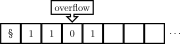
\includegraphics{res/turing_add1_4.svg}
\caption{\(δ(s_\text{overflow}, \zer) = (s_\text{return}, \one, -1)\)}
\end{figure}

\begin{figure}
\centering
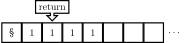
\includegraphics{res/turing_add1_5.svg}
\caption{\(δ(s_\text{return}, \one) = (s_\text{return}, \one, -1)\)}
\end{figure}

\begin{figure}
\centering
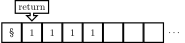
\includegraphics{res/turing_add1_6.svg}
\caption{\(δ(s_\text{return}, \one) = (s_\text{return}, \one, -1)\)}
\end{figure}

\begin{figure}
\centering
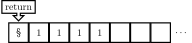
\includegraphics{res/turing_add1_7.svg}
\caption{\(δ(s_\text{return}, \sta) = (s_\text{halt}, \sta, 0)\)}
\end{figure}

\begin{figure}
\centering
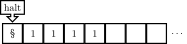
\includegraphics{res/turing_add1_8.svg}
\caption{\(δ(s_\text{halt}, \sta) = (s_\text{halt}, \sta, 0)\)}
\end{figure}

The complete run of \(\mathbb A_\text{add1}\) on \(\one\one\zer\one\)

Let \(\mathbb A\) be a Turing machine.

\begin{enumerate}
\def\labelenumi{\arabic{enumi}.}
\tightlist
\item
  \(\mathbb A\) \emph{computes} the partial function that maps each
  \(x\) with a complete run to \(\mathbb A(x)\) and is undefined for all
  other strings.
\item
  \(\mathbb A\) \emph{accepts} all \(x\) such that
  \(\mathbb A(x) = \one\) and \emph{rejects} them if
  \(\mathbb A(x) = \zer\).
\item
  A partial function on \(\lbrace \sta, \emp, \zer, \one \rbrace^*\) is
  \emph{computable} if there is a Turing machine computing it.
\item
  A subset of \(\lbrace \sta, \emp, \zer, \one \rbrace^*\), i.e.~a
  problem, is \emph{decidable} if there is a Turing machine computing
  its characteristic function.
\item
  A problem is called \emph{semi-decidable} or \emph{computably
  enumerable} if there is a Turing machine accepting precisely the
  elements of the problem.
\end{enumerate}

The last postulate of the definition above means that a problem is
semi-decidable if there is a Turing machine affirming membership of the
corresponding set but it might not be able to refute membership.

We can encode a natural number \(n\)

\begin{enumerate}
\def\labelenumi{\arabic{enumi}.}
\tightlist
\item
  in tally notation \[n ↦ \underbrace{\one…\one}_{n\text{-times}},\]
\item
  by its binary representation
  \[n = 2^k + \sum_{i = 0}^{k-1} b_i 2^i ↦ b_0…b_{k-1}\one,\]
  \[0 ↦ \zer \text{, or}\]
\item
  by a shifted and truncated form of its binary representation
  \[n = 1 + \sum_{i = 0}^k b_i 2^i ↦ b_0…b_{k-1},\] \[0 ↦ λ\]
\end{enumerate}

In either case the set obtained by encoding \(ℕ\) is easily seen to be
decidable. In the first case, check that the string contains only copies
of the bit \(\one\).

This can be achieved by the Turing machine
\(\mathbb A_\text{tally} = ( \lbrace \sstart, \shalt, \scheck, s_\text{accept}, s_\text{reject}, s_\text{rejectMR}\rbrace, δ)\)
with

\begin{Shaded}
\begin{Highlighting}[]
\CommentTok{-- start by entering the "check" state and ...}
\NormalTok{tally }\StringTok{"start"}    \CharTok{'§'}    \FunctionTok{=}\NormalTok{ (}\StringTok{"check"}\NormalTok{,    }\CharTok{'§'}\NormalTok{, }\DecValTok{1}\NormalTok{   )}
\CommentTok{-- ... stay in this state while reading only '1'-s}
\NormalTok{tally }\StringTok{"check"}    \CharTok{'1'}    \FunctionTok{=}\NormalTok{ (}\StringTok{"check"}\NormalTok{,    }\CharTok{'1'}\NormalTok{, }\DecValTok{1}\NormalTok{   )}
\CommentTok{-- on reading '□' accept the input and clear the tape ...}
\NormalTok{tally }\StringTok{"check"}    \CharTok{'□'}    \FunctionTok{=}\NormalTok{ (}\StringTok{"accept"}\NormalTok{,   }\CharTok{'□'}\NormalTok{, (}\FunctionTok{-}\DecValTok{1}\NormalTok{))}
\NormalTok{tally }\StringTok{"accept"}   \CharTok{'1'}    \FunctionTok{=}\NormalTok{ (}\StringTok{"accept"}\NormalTok{,   }\CharTok{'□'}\NormalTok{, (}\FunctionTok{-}\DecValTok{1}\NormalTok{))}
\CommentTok{-- ...except for cell c(1) where you write a '1'}
\NormalTok{tally }\StringTok{"accept"}   \CharTok{'§'}    \FunctionTok{=}\NormalTok{ (}\StringTok{"accept"}\NormalTok{,   }\CharTok{'§'}\NormalTok{, }\DecValTok{1}\NormalTok{   )}
\NormalTok{tally }\StringTok{"accept"}   \CharTok{'□'}    \FunctionTok{=}\NormalTok{ (}\StringTok{"halt"}\NormalTok{,     }\CharTok{'1'}\NormalTok{, (}\FunctionTok{-}\DecValTok{1}\NormalTok{))}
\CommentTok{-- however, if you read a '0' first reject the input}
\CommentTok{-- by moving to the end of the input string ...}
\NormalTok{tally }\StringTok{"check"}    \CharTok{'0'}    \FunctionTok{=}\NormalTok{ (}\StringTok{"rejectMR"}\NormalTok{, }\CharTok{'0'}\NormalTok{, }\DecValTok{1}\NormalTok{   )}
\NormalTok{tally }\StringTok{"rejectMR"} \CharTok{'□'}    \FunctionTok{=}\NormalTok{ (}\StringTok{"reject"}\NormalTok{,   }\CharTok{'□'}\NormalTok{, (}\FunctionTok{-}\DecValTok{1}\NormalTok{))}
\NormalTok{tally }\StringTok{"rejectMR"}\NormalTok{ b      }\FunctionTok{=}\NormalTok{ (}\StringTok{"rejectMR"}\NormalTok{, b,   }\DecValTok{1}\NormalTok{   ) }\CommentTok{-- `b` is '0' or '1'}
\CommentTok{-- ... and clear the tape except for cell c(1) where you}
\CommentTok{-- write a '0'}
\NormalTok{tally }\StringTok{"reject"}   \CharTok{'§'}    \FunctionTok{=}\NormalTok{ (}\StringTok{"reject"}\NormalTok{,   }\CharTok{'§'}\NormalTok{, }\DecValTok{1}\NormalTok{   )}
\NormalTok{tally }\StringTok{"reject"}   \CharTok{'□'}    \FunctionTok{=}\NormalTok{ (}\StringTok{"halt"}\NormalTok{,     }\CharTok{'0'}\NormalTok{, (}\FunctionTok{-}\DecValTok{1}\NormalTok{))}
\NormalTok{tally }\StringTok{"reject"}\NormalTok{   b      }\FunctionTok{=}\NormalTok{ (}\StringTok{"reject"}\NormalTok{,   }\CharTok{'□'}\NormalTok{, (}\FunctionTok{-}\DecValTok{1}\NormalTok{)) }\CommentTok{-- `b` is '0' or '1'}
\end{Highlighting}
\end{Shaded}

In the second case it suffices to check that the string has length \(1\)
or ends in a \(\one\), and in the third case every string is accepted.

\subsubsection{Halting problem}\label{halting-problem}

One can extend the alphabet of Turing machines by encoding characters
i.e.~assigning bit sequences to them. Very common encodings are
\emph{ASCII} and \emph{UTF-8}\footnote{See the Appendix for an
  \emph{ASCII} encoding table and details on \emph{UTF-8}.}. Using
either one of these encodings the string `haskell' is encoded as

\begin{verbatim}
h         a         s         k         e         l         l
0110 1000 0110 0001 0111 0011 0110 1011 0110 0101 0110 1100 0110 1100
\end{verbatim}

In this way we can encode a Turing machine as the UTF-8--encoding of
their transition function \(δ\) written as a string as above. Note that
the set of states can implicitly be deduced from the transition function
as the set of acceptable first arguments of \(δ\).

One of the fundamental theorems of theoretical computer science is the
existence of a universal Turing machine.

There exists a Turing machine \(\mathbb U\) that computes upon receiving
the tuple \((\ulcorner \mathbb A \urcorner, x)\) as input, the output of
Turing machine \(\mathbb A\) on \(x\) i.e.
\[ \mathbb U(\ulcorner \mathbb A \urcorner, x) = y \Leftrightarrow \mathbb A (x) = y\]

A natural question is:

Given a machine \(\mathbb A\) and a string \(x\). Does \(\mathbb A\)
halt on \(x\)?

It is one of the most fundamental results of theoretical computer
science that the halting problem is unsolvable.

The halting problem is undecidable.

Assume there exists a Turing machine \(\mathbb B\) that decides the
halting problem i.e.~for all Turing machines \(\mathbb A\) and all
strings \(x\)

\[ \mathbb B(\mathbb A, x) =
\begin{cases}
  \one  & \text{if } \mathbb A \text{ halts on } x\\
  \zer  & \text{if } \mathbb A \text{ does not halt on } x
\end{cases}\]

Now using \(\mathbb B\) construct a Turing machine \(\mathbb B'\) such
that

\[ \mathbb B'(\mathbb A) = \one \Leftrightarrow \mathbb A \text{ does not halt on } \ulcorner \mathbb A\urcorner \]

Now if \(\mathbb B'(\mathbb B, \ulcorner \mathbb B\urcorner) = \one\)
then by definition of \(\mathbb B'\) we find that
\(\mathbb B does not halt on \ulcorner \mathbb B\urcorner\). But by
definiton of \(\mathbb B\) this means that
\(\mathbb B(\mathbb B, \ulcorner \mathbb B \urcorner) = \zer\)
